% Provenance (never printed): cycle 2 "Questionner l'espace et le temps"
% (oceans, seas, continents on the globe) and "Questionner le monde de la
% matiere" (states of water in natural phenomena); see sources/book1/PROVENANCE.md.
% Book 1, grade 2, chapter 1.
\chapter{الماء على الأرض}\label{ch:g2:water-on-earth}

في السابع من ديسمبر سنة 1972، أدار ثلاثة رواد فضاء في طريقهم إلى القمر
آلة تصويرهم نحو الأرض. فصارت صورتهم من أشهر الصور التي التُقطت في
التاريخ. انظر إليها. ترى غيومًا بيضاء، وقليلًا من اليابسة البنية
والصفراء، والجليد الأبيض في الأسفل --- وزرقة، زرقة في كل مكان. كوكبنا،
إذا نظرنا إليه من الفضاء، كوكب أزرق.

\begin{omfigure}
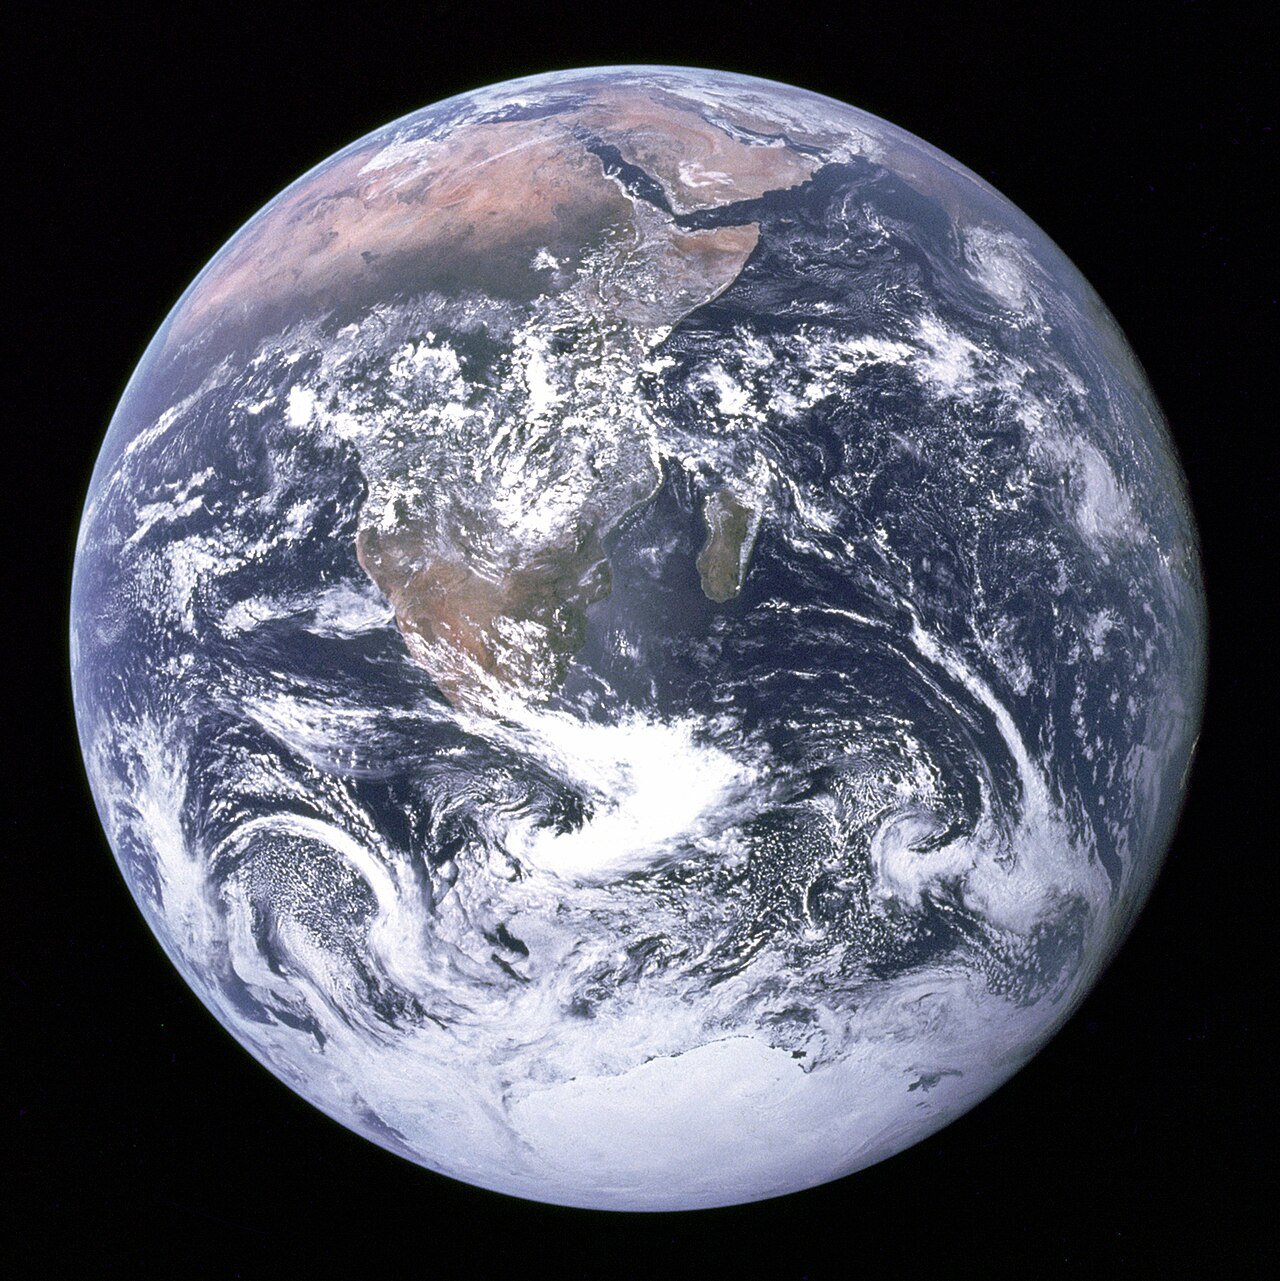
\includegraphics[width=0.5\linewidth]{images/book1/g2-nasa-blue-marble.jpg}

{\small الأرض كما صوّرها طاقم أبولو~17، في 7~ديسمبر 1972. نرى إفريقيا،
وشبه الجزيرة العربية في الأعلى، وجليد القارة القطبية الجنوبية في الأسفل.
الصورة: ناسا (ملك عام).}
\end{omfigure}

\begin{recall}
يمكن أن يكون الماء صلبًا (جليدًا)، أو سائلًا، أو غازًا لا نراه (بخار
الماء). الماء السائل المتروك في الشمس يتحول ببطء إلى بخار: إنه يتبخر.
وحين يبرد البخار يعود قطرات صغيرة جدًا: إنه يتكاثف. وقد تعرفت هذه
التحولات في كتب الفيزياء. وفي \omterm{def:g1:landscapes-around-us:landscape}{المنظر}، يجري الماء في \omterm{def:g1:landscapes-around-us:water}{الأنهار} ويستقر في
\omterm{def:g1:landscapes-around-us:water}{البحيرات} (\cref{ch:g1:landscapes-around-us}).
\end{recall}

\section{الكوكب الأزرق}

معظم الأرض يغطيه الماء. تخيل أننا قسمنا سطح الأرض كله إلى 100 مربع
متساوٍ. إذا لوّنا بالأزرق كل مربع يغطيه \omterm{def:g2:water-on-earth:ocean}{البحر}، فسنلوّن 71 مربعًا. ولا
يبقى لليابسة إلا 29 مربعًا.

\begin{omfigure}
\begin{tikzpicture}
  \begin{axis}[hide axis, width=7.2cm, height=7.2cm, xmin=-0.5, xmax=9.5,
      ymin=-0.5, ymax=9.5, axis equal image, scale only axis,
      clip=false]
    \addplot[scatter, only marks, mark=square*, mark size=9.2pt,
      scatter/classes={0={fill=green!45!omLithAlluv, draw=black!40},
                       1={fill=omSea!80!blue, draw=black!40}},
      point meta=explicit symbolic]
      table[x=col, y=row, meta=blue] {figdata/out/grade-2-ocean_fraction-grid.dat};
  \end{axis}
\end{tikzpicture}

{\small لو قُسم سطح الأرض إلى 100 مربع متساوٍ، لكان 71 منها بحرًا (أزرق)
و29 يابسة (أخضر). حُسبت من خريطة لتضاريس الأرض كلها (NOAA
ETOPO1).}
\label{fig:g2:water-on-earth:grid}
\end{omfigure}
% ledger: data:etopo1, wss:ocean-cover (71 % computed in figdata/grade-2/ocean_fraction.py)

للمساحات الواسعة من \omterm{def:g2:water-on-earth:salt-fresh}{الماء المالح} التي تغطي معظم الأرض أسماء.

\begin{definition}[المحيط والبحر]\label{def:g2:water-on-earth:ocean}
\emph{المحيط}\index{محيط} واحد من المساحات الواسعة جدًا من \omterm{def:g2:water-on-earth:salt-fresh}{الماء المالح}
التي تغطي معظم الأرض وتقع بين القارات.
و\emph{البحر}\index{بحر} مساحة أصغر من \omterm{def:g2:water-on-earth:salt-fresh}{الماء المالح}، تقع عادة على
طرف محيط وتحيط بها اليابسة من بعض جهاتها.
\end{definition}

المحيطات كلها متصل بعضها ببعض: يستطيع مركب أن يبحر من أي \omterm{def:g2:water-on-earth:ocean}{محيط} إلى أي
\omterm{def:g2:water-on-earth:ocean}{محيط} آخر دون أن يعبر يابسة. وأسماؤها، ومواقعها على الكرة الأرضية، في
\cref{ch:g3:continents-and-oceans}.

\begin{omfigure}
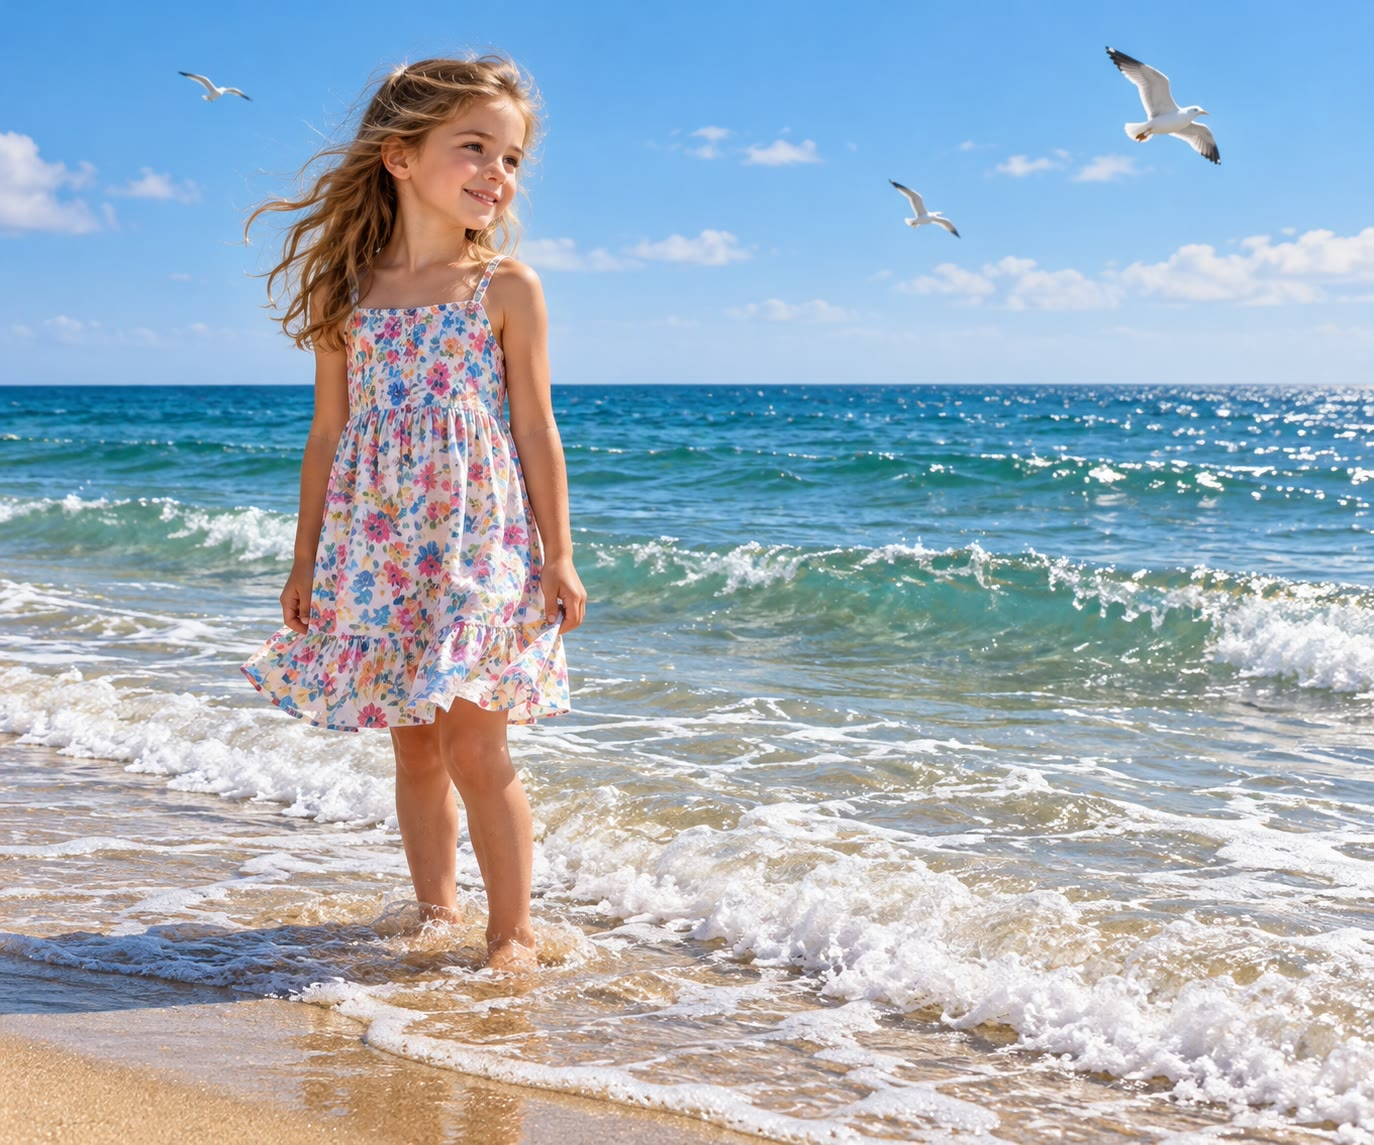
\includegraphics[width=0.62\linewidth]{images/book1/ai/g2-beach-sea.jpg}

{\small على شاطئ \omterm{def:g2:water-on-earth:ocean}{البحر}. يمتد الماء أبعد بكثير مما تراه
العين.}
\end{omfigure}

\section{الماء المالح والماء العذب}

إذا كنت قد ابتلعت يومًا جرعة من ماء \omterm{def:g2:water-on-earth:ocean}{البحر} وأنت تسبح، فأنت تعرف: طعمه
مالح جدًا. أما ماء \omterm{def:g1:landscapes-around-us:water}{الأنهار} \omterm{def:g1:landscapes-around-us:water}{والبحيرات} فليس كذلك.

\begin{definition}[الماء المالح والماء العذب]\label{def:g2:water-on-earth:salt-fresh}
\emph{الماء المالح}\index{ماء مالح} ماء ذاب فيه كثير من الملح: هو ماء
المحيطات والبحار. و\emph{الماء العذب}\index{ماء عذب}
فيه قليل جدًا من الملح: هو ماء المطر، وأكثر \omterm{def:g1:landscapes-around-us:water}{الأنهار} \omterm{def:g1:landscapes-around-us:water}{والبحيرات}،
والجليد والثلج، والينابيع.
\end{definition}

\begin{example}[ما مقدار ملوحة البحر؟]\label{ex:g2:water-on-earth:salty}
% ledger: nos:salinity
في قارورة فيها كيلوغرام واحد من ماء \omterm{def:g2:water-on-earth:ocean}{البحر} --- نحو لتر واحد --- يوجد
نحو 35 غرامًا من الملح. وإذا تركنا الماء كله يتبخر، يبقى الملح بلورات
بيضاء في القاع. وهكذا يُصنع ملح \omterm{def:g2:water-on-earth:ocean}{البحر} في الملاحات على شاطئ \omterm{def:g2:water-on-earth:ocean}{البحر}، حيث
تجفف الشمس والريح ببطء أحواضًا ضحلة من ماء
\omterm{def:g2:water-on-earth:ocean}{البحر}.
\end{example}

\begin{omfigure}
\begin{minipage}[b]{0.49\linewidth}\centering
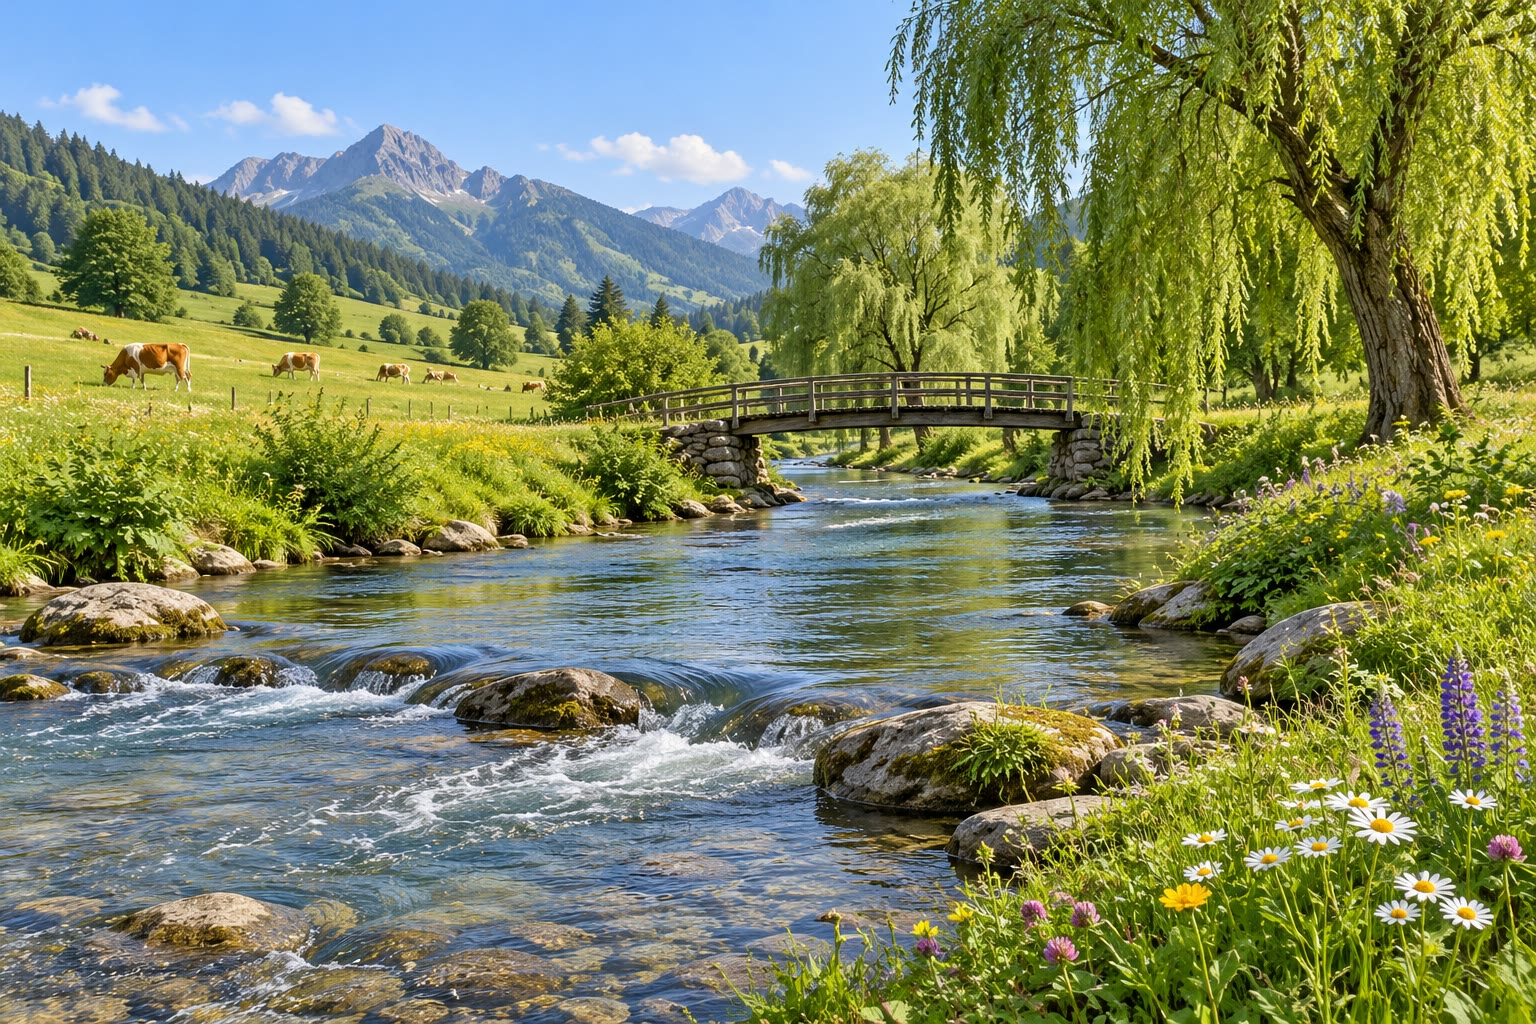
\includegraphics[width=\linewidth]{images/book1/ai/g2-river-meadow.jpg}

{\small \omterm{def:g2:water-on-earth:salt-fresh}{ماء عذب}: \omterm{def:g1:landscapes-around-us:water}{نهر}.}
\end{minipage}\hfill
\begin{minipage}[b]{0.49\linewidth}\centering
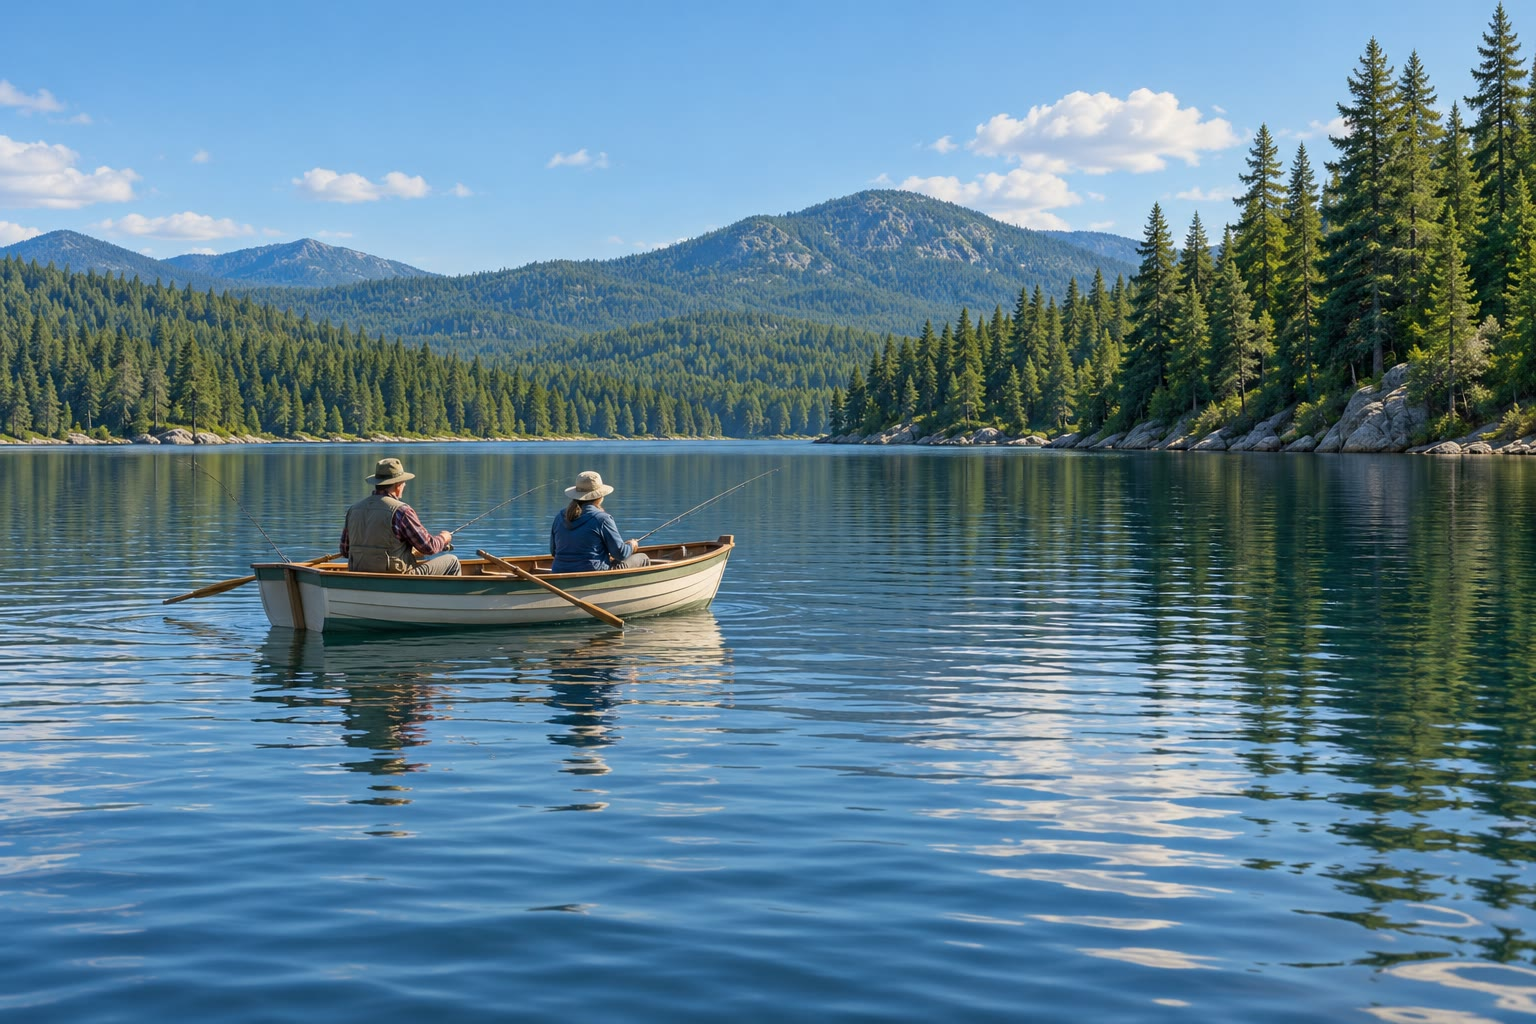
\includegraphics[width=\linewidth]{images/book1/ai/g2-lake-boat.jpg}

{\small \omterm{def:g2:water-on-earth:salt-fresh}{ماء عذب}: \omterm{def:g1:landscapes-around-us:water}{بحيرة}.}
\end{minipage}
\end{omfigure}

\begin{remark}[لا نستطيع شرب ماء البحر]\label{rem:g2:water-on-earth:drink}
لا يستطيع الناس ولا حيوانات اليابسة شرب ماء \omterm{def:g2:water-on-earth:ocean}{البحر}: ففيه ملح كثير جدًا،
وشربه يجعل الجسم يفقد الماء بدل أن يكسبه. والبحارة في عرض \omterm{def:g2:water-on-earth:ocean}{البحر}،
والماء يحيط بهم من كل جانب، كان عليهم دائمًا أن يحملوا معهم ماءهم
العذب.
\end{remark}

\section{أين يوجد الماء كله؟}

\omterm{def:g2:water-on-earth:salt-fresh}{الماء العذب} لا يوجد في \omterm{def:g1:landscapes-around-us:water}{الأنهار} \omterm{def:g1:landscapes-around-us:water}{والبحيرات} فقط. فكثير منه متجمد: في الجليد
الأبيض العظيم في القارة القطبية الجنوبية وغرينلاند، وعلى \omterm{def:g1:landscapes-around-us:landform}{الجبال} العالية.
وكثير منه مختبئ تحت أقدامنا، في باطن الأرض، حيث يملأ الفراغات الصغيرة
جدًا بين حبيبات الرمل وشقوق الصخر.

\begin{omfigure}
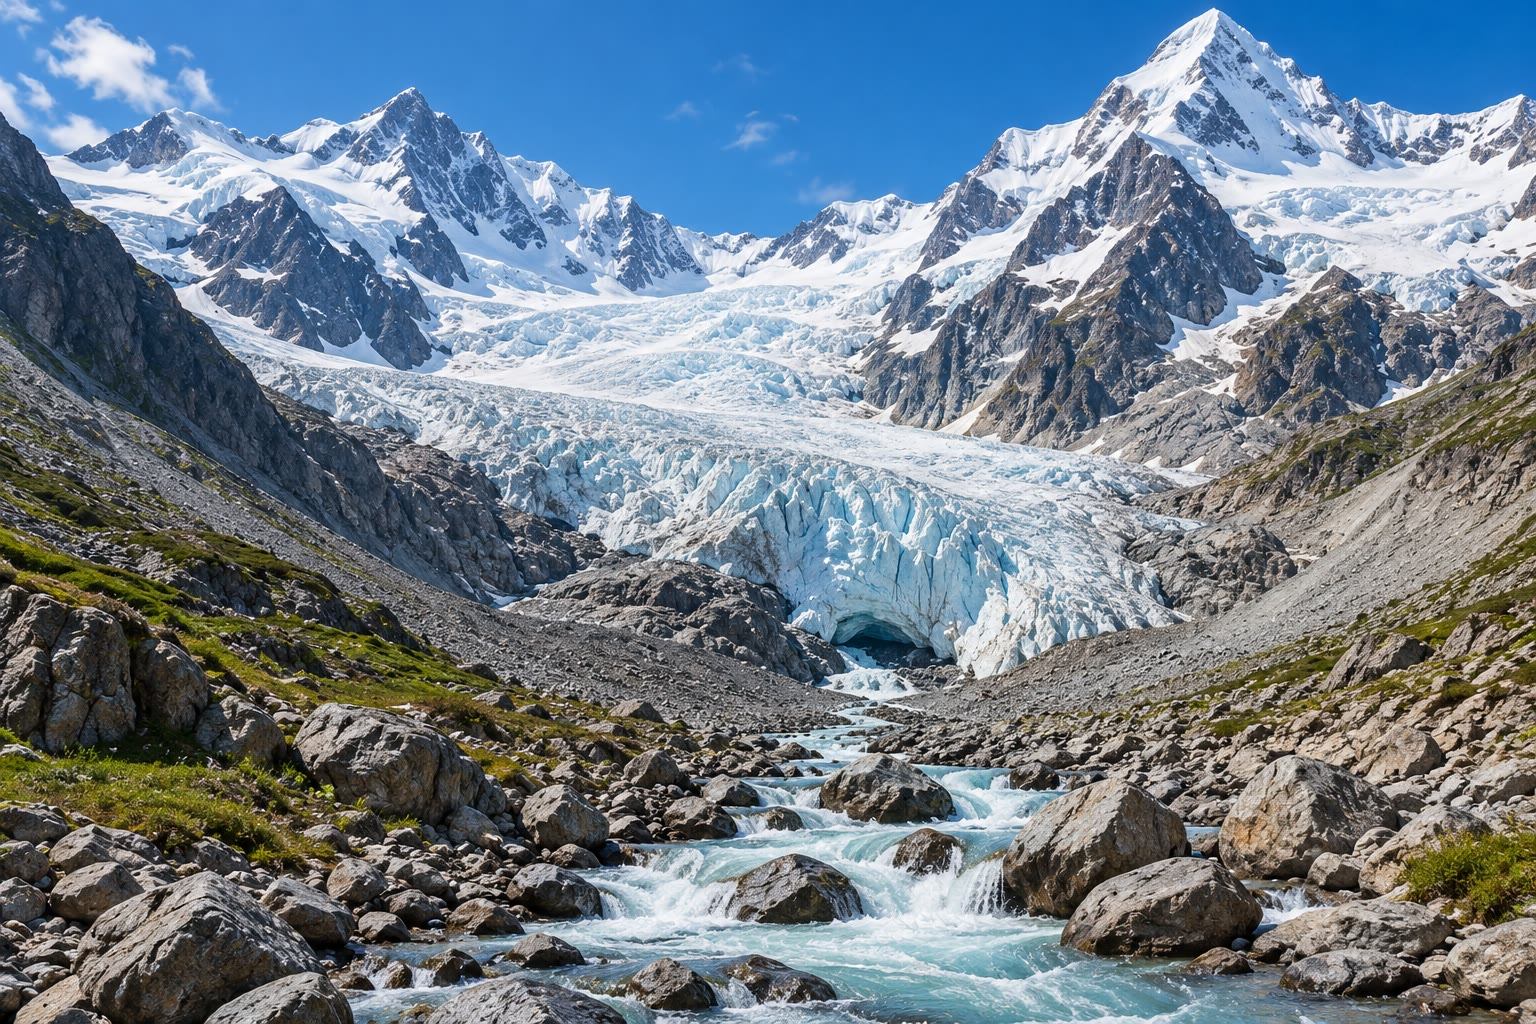
\includegraphics[width=0.62\linewidth]{images/book1/ai/g2-snowy-mountains.jpg}

{\small تحفظ \omterm{def:g1:landscapes-around-us:landform}{الجبال} العالية \omterm{def:g2:water-on-earth:salt-fresh}{الماء العذب} ثلجًا وجليدًا طوال السنة. وفي
الصيف يذوب بعضه ويغذي الجداول.}
\end{omfigure}

تخيل أننا نستطيع أن نصب ماء الأرض كله في 100 دلو من الحجم نفسه. كم دلوًا
يملأ كل نوع من الماء؟

\begin{omfigure}
\begin{tikzpicture}
  \begin{axis}[hide axis, width=7.2cm, height=7.2cm, xmin=-0.5, xmax=9.5,
      ymin=-0.5, ymax=9.5, axis equal image, scale only axis, clip=false]
    \addplot[scatter, only marks, mark=*, mark size=8pt,
      scatter/classes={0={fill=omSea!80!blue, draw=black!40},
                       1={fill=white, draw=black!60},
                       2={fill=brown!55, draw=black!40}},
      point meta=explicit symbolic]
      table[x=col, y=row, meta=kind] {figdata/out/grade-2-water_shares.dat};
  \end{axis}
  \begin{scope}[shift={(7.9,5.6)}, font=\small]
    \fill[omSea!80!blue, draw=black!40] (0,0) circle (0.2);
    \node[anchor=west] at (0.35,0) {\foreignlanguage{arabic}{الماء المالح في المحيطات: \babelsublr{96} دلوًا}};
    \fill[white, draw=black!60] (0,-0.7) circle (0.2);
    \node[anchor=west] at (0.35,-0.7) {\foreignlanguage{arabic}{الجليد والثلج: دلوان}};
    \fill[brown!55, draw=black!40] (0,-1.4) circle (0.2);
    \node[anchor=west] at (0.35,-1.4) {\foreignlanguage{arabic}{الماء تحت الأرض: دلوان}};
  \end{scope}
\end{tikzpicture}

{\small ماء الأرض كله في 100 دلو. \omterm{def:g1:landscapes-around-us:water}{الأنهار} \omterm{def:g1:landscapes-around-us:water}{والبحيرات} والغيوم وماء الكائنات
الحية كلها معًا لا تملأ دلوًا واحدًا. الأرقام من هيئة المسح الجيولوجي
الأمريكية.}
\label{fig:g2:water-on-earth:buckets}
\end{omfigure}
% ledger: wss:water-shares (rounded to 100 buckets in figdata/grade-2/water_shares.py)

\begin{proposition}[معظم ماء الأرض مالح]\label{prop:g2:water-on-earth:most-salty}
% ledger: wss:water-shares
من بين 100 دلو تحمل ماء الأرض كله، 96 دلوًا هي \omterm{def:g2:water-on-earth:salt-fresh}{الماء المالح} في المحيطات.
\omterm{def:g2:water-on-earth:salt-fresh}{والماء العذب} الذي نشربه ليس إلا جزءًا صغيرًا جدًا من الماء كله: معظمه
متجمد في الجليد، أو مختبئ تحت الأرض.
\end{proposition}

\section{إلى أين يذهب المطر؟}

حين تمطر لا يبقى الماء حيث يسقط. راقب ساحة المدرسة بعد زخة مطر: بعض
الماء يجري على الأرض إلى المزاريب، وبعضه يتسرب في تربة أحواض الزهور،
والبرك تختفي ببطء حين تعود الشمس.

\begin{omfigure}
\begin{tikzpicture}[x=1cm, y=1cm, font=\small]
  % sky, sea, land
  \fill[ocBlue!6] (0,0) rectangle (12,5.6);
  \fill[omSea] (8.6,0) rectangle (12,0.9);
  \fill[green!30!omLithAlluv] (0,0) -- (0,2.4) .. controls (2,2.6) and (3,2.0) .. (4.5,1.6)
     .. controls (6,1.2) and (7.5,1.0) .. (8.6,0.9) -- (8.6,0) -- cycle;
  % ground below the surface
  \fill[brown!25] (0,0) rectangle (8.6,0.6);
  % river
  \draw[omSea!70!blue, line width=2.4pt] (1.6,2.45) .. controls (3.5,2.0) and (6,1.15) .. (8.6,0.95);
  % cloud and rain
  \pic at (2.2,4.0) {puffycloud};
  \foreach \x in {1.4,1.8,2.2,2.6,3.0}
    \draw[omWxRain, line width=0.8pt] (\x,3.7) -- (\x-0.15,3.1);
  \pic at (9.6,4.3) {puffycloud};
  % arrows
  \draw[omWxRain, line width=1.1pt, -{Stealth[length=2.5mm]}] (3.3,2.15) -- (3.3,0.6);
  \node[anchor=west, align=left, font=\scriptsize] at (3.4,1.0) {بعضه يتسرب\\في الأرض};
  \draw[omWxRain, line width=1.1pt, -{Stealth[length=2.5mm]}] (5.4,1.55) -- (7.6,1.15);
  \node[align=center, font=\scriptsize] at (6.2,2.05) {بعضه يجري إلى نهر\\والنهر يجري إلى البحر};
  \draw[black!50, line width=1.1pt, densely dashed, -{Stealth[length=2.5mm]}] (10.2,1.1) .. controls (10.4,2.4) and (10.1,3.2) .. (9.8,3.85);
  \node[align=left, anchor=west, font=\scriptsize] at (10.45,2.4) {الماء\\يتبخر};
  \draw[black!50, line width=1.1pt, densely dashed, -{Stealth[length=2.5mm]}] (8.45,4.35) -- (3.6,4.3);
  \node[font=\scriptsize, above] at (6.0,4.35) {الريح تحمل الغيوم};
  \node[font=\scriptsize] at (10.4,0.45) {البحر};
  \node[font=\scriptsize, anchor=west] at (0.2,3.25) {المطر};
\end{tikzpicture}

{\small إلى أين يذهب المطر. الماء الذي يصعد بخارًا من \omterm{def:g2:water-on-earth:ocean}{البحر} ومن اليابسة
يصنع غيومًا جديدة، والغيوم تأتي بمطر جديد.}
\label{fig:g2:water-on-earth:rain}
\end{omfigure}

\begin{method}[تتبع قطرة مطر]\label{met:g2:water-on-earth:drop}
لتتبع قطرة مطر، اطرح ثلاثة أسئلة واحدًا بعد الآخر:
\begin{enumerate}
  \item أين تسقط: على \omterm{def:g2:water-on-earth:ocean}{البحر}، على سطح بيت، على التربة، على
        \omterm{def:g1:landscapes-around-us:landform}{جبل}؟
  \item هل تتسرب في الأرض، أم تجري على السطح، أم تتجمد
        فتصير جليدًا؟
  \item إلى أين تذهب بعد ذلك: إلى \omterm{def:g1:landscapes-around-us:water}{نهر}، أو \omterm{def:g1:landscapes-around-us:water}{بحيرة}، أو \omterm{def:g2:water-on-earth:ocean}{البحر}، أو باطن الأرض،
        أو تعود إلى الهواء؟
\end{enumerate}
في النهاية تعود كل قطرة إلى \omterm{def:g2:water-on-earth:ocean}{البحر} أو إلى الهواء، وتبدأ الرحلة من
جديد.
\end{method}

\begin{example}[قطرة على الجبل]\label{ex:g2:water-on-earth:mountain}
تسقط قطرة مطر ثلجًا على \omterm{def:g1:landscapes-around-us:landform}{جبل} عالٍ في الشتاء. وتبقى هناك متجمدة حتى أيام
الصيف الدافئة. ثم تذوب، وتنحدر في جدول جبلي، وتلتحق \omterm{def:g1:landscapes-around-us:water}{بنهر}، فيحملها \omterm{def:g1:landscapes-around-us:water}{النهر}
إلى \omterm{def:g2:water-on-earth:ocean}{البحر}. وفي يوم مشمس تتبخر القطرة من \omterm{def:g2:water-on-earth:ocean}{البحر} وتصعد في الهواء، فتصير
جزءًا من غيمة جديدة.
\end{example}

\section{تمارين}

\begin{exercise}[$\star$]\label{exo:g2:water-on-earth:1}
\omterm{def:g2:water-on-earth:salt-fresh}{ماء مالح} أم \omterm{def:g2:water-on-earth:salt-fresh}{ماء عذب}؟ \omterm{def:g2:water-on-earth:ocean}{البحر}؛ \omterm{def:g1:landscapes-around-us:water}{نهر}؛ المطر؛ \omterm{def:g1:landscapes-around-us:water}{بحيرة} في \omterm{def:g1:landscapes-around-us:landform}{الجبال}؛ \omterm{def:g2:water-on-earth:ocean}{محيط}؛ الجليد
على \omterm{def:g1:landscapes-around-us:landform}{جبل}.
\end{exercise}

\begin{exercise}[$\star$]\label{exo:g2:water-on-earth:2}
لماذا نسمي الأرض «الكوكب الأزرق»؟
\end{exercise}

\begin{exercise}[$\star$]\label{exo:g2:water-on-earth:3}
في شبكة المربعات المئة، 71 مربعًا زرقاء. كم مربعًا
يابسة؟
\end{exercise}

\begin{exercise}[$\star$]\label{exo:g2:water-on-earth:4}
أيهما أكبر، \omterm{def:g2:water-on-earth:ocean}{المحيط} أم \omterm{def:g2:water-on-earth:ocean}{البحر}؟
\end{exercise}

\begin{exercise}[$\star$]\label{exo:g2:water-on-earth:5}
هل يستطيع بحار في وسط \omterm{def:g2:water-on-earth:ocean}{المحيط} أن يشرب الماء الذي حول المركب؟
لماذا؟
\end{exercise}

\begin{exercise}[$\star$]\label{exo:g2:water-on-earth:6}
سمِّ ثلاثة أماكن يوجد فيها \omterm{def:g2:water-on-earth:salt-fresh}{الماء العذب}.
\end{exercise}

\begin{exercise}[$\star\star$]\label{exo:g2:water-on-earth:7}
في صورة الدلاء المئة، كم دلوًا من \omterm{def:g2:water-on-earth:salt-fresh}{الماء المالح}؟ وكم دلوًا من \omterm{def:g2:water-on-earth:salt-fresh}{الماء العذب}
(الجليد والماء تحت الأرض معًا)؟
\end{exercise}

\begin{exercise}[$\star\star$]\label{exo:g2:water-on-earth:8}
رتّب ما يلي، من الذي يحوي أكثر الماء إلى الذي يحوي أقله: \omterm{def:g1:landscapes-around-us:water}{الأنهار}؛
المحيطات؛ الجليد والثلج.
\end{exercise}

\begin{exercise}[$\star\star$]\label{exo:g2:water-on-earth:9}
تمطر على حقل. اذكر أمرين يمكن أن يحدثا للماء.
\end{exercise}

\begin{exercise}[$\star\star$]\label{exo:g2:water-on-earth:10}
تُرك وعاء فيه ماء \omterm{def:g2:water-on-earth:ocean}{البحر} في الشمس أيامًا كثيرة، حتى ذهب الماء. ماذا بقي في
قاع الوعاء؟ وإلى أين ذهب الماء؟
\end{exercise}

\begin{exercise}[$\star\star$]\label{exo:g2:water-on-earth:11}
احكِ رحلة قطرة مطر تسقط على سطح المدرسة، حتى تعود إلى
غيمة.
\end{exercise}
